\begin{figure}[htbp]
	% Partly taken from http://www.texample.net/tikz/examples/convolution-of-two-functions/
	\centering
	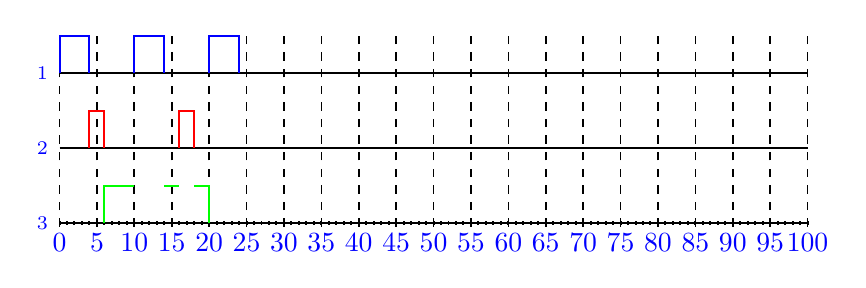
\begin{tikzpicture}[
		scale=0.095,
		line width=0.25mm,
		every node/.style={scale=1, text=blue},
		major tick/.style={semithick, dashed},
		x tick label/.style={anchor=north, minimum width=5mm},
		task1/.style={blue},
		task2/.style={red},
		task3/.style={green},
		desc/.style={anchor=east}
		]		

	% Task 1
	\draw (0, 20) -- (100, 20);
	\node[desc] at (0, 20) {$\uptau_1$};		
	
	% Task 2
	\draw (0, 10) -- (100, 10);
	\node[desc] at (0, 10) {$\uptau_2$};	
	
	% Task 3
	\draw (0, 0) -- (100, 0);
	\node[desc] at (0, 0) {$\uptau_3$};	
	
	% Small ticks
	\foreach \x in {0, 1,...,100}{
		\draw (\x, -0.25) -- (\x, 0.25);
	}
	
	% Major ticks with label
	\foreach \x/\label in {0, 5,...,100}{
		\node[x tick label] at (\x, 0) {$\label$}; 		
		\draw[major tick] (\x, -0.5) -- (\x, 26);
	}
	
	\draw[task1] (0, 20) -- (0, 25) -- (4, 25) -- (4, 20);
	\draw[task2] (4, 10) -- (4, 15) -- (6, 15) -- (6, 10);
	\draw[task3] (6, 0) -- (6, 5) -- (10, 5); % 4 of 8
	\draw[task1] (10, 20) -- (10, 25) -- (14, 25) -- (14, 20);
	\draw[task3] (14, 5) -- (16, 5); % 6 of 8
	\draw[task2] (16, 10) -- (16, 15) -- (18, 15) -- (18, 10);
	\draw[task3] (18, 5) -- (20, 5) -- (20, 0); % 8 of 8
	\draw[task1] (20, 20) -- (20, 25) -- (24, 25) -- (24, 20);
%	
%	\draw[task3] (24, 0) -- (24, 5) -- (30, 5); % 6 of 8
%	\draw[task1] (30, 20) -- (30, 25) -- (34, 25) -- (34, 20);
%	\draw[task2] (34, 10) -- (34, 15) -- (36, 15) -- (36, 10);
%	\draw[task3] (36, 5) -- (38, 5) -- (38, 0); % 8 of 8
%	\draw[task1] (40, 20) -- (40, 25) -- (44, 25) -- (44, 20);
%	\draw[task3] (44, 0) -- (44, 5) -- (48, 5); % 4 of 8	
%	\draw[task2] (48, 10) -- (48, 15) -- (50, 15) -- (50, 10);
%	\draw[task1] (50, 20) -- (50, 25) -- (54, 25) -- (54, 20);
%	\draw[task3] (50, 5) -- (54, 5) -- (54, 0); % 8 of 8	
%	
%	\draw[task1] (60, 20) -- (60, 25) -- (64, 25) -- (64, 20);
%	\draw[task2] (64, 10) -- (64, 15) -- (66, 15) -- (66, 10);
%	\draw[task3] (66, 0) -- (66, 5) -- (70, 5); % 4 of 8
%	\draw[task1] (70, 20) -- (70, 25) -- (74, 25) -- (74, 20);
%	\draw[task3] (74, 5) -- (78, 5) -- (78, 0); % 8 of 8
%	
%	\draw[task1] (80, 20) -- (80, 25) -- (84, 25) -- (84, 20);
%	\draw[task2] (84, 10) -- (84, 15) -- (86, 15) -- (86, 10);
%	\draw[task3] (86, 0) -- (86, 5) -- (90, 5); % 4 of 8
%	\draw[task1] (90, 20) -- (90, 25) -- (94, 25) -- (94, 20);
%	\draw[task3] (94, 5) -- (96, 5); % 6 of 8
%	\draw[task2] (96, 10) -- (96, 15) -- (98, 15) -- (98, 10);
%	\draw[task3] (98, 5) -- (100, 5) -- (100, 0); % 8 of 8
		
	\end{tikzpicture}
%	\caption{Ablaufübersicht}
\end{figure} 